\section{\trCofinal{}与\trCoinitial{}函子}
\label{sec:cofinal-coinitial-functors}

在本节中，我们讨论\trCofinal{}与\trCoinitial{}函子的概念。非形式地讲，它们是那类%
\trFunctor{} $f\colon I \to J$：无论图表 $J \to \C$ 如何选取，它们分别在%
\trColimit{}与\trLimit{}上诱导出等价。借助\trCofinal{}与\trCoinitial{}函子，
我们将讨论\trSmooth{}（smooth）与\trProper{}（proper）\trFunctor{}的概念，
并证明\trLeftFibration{}都是\trSmooth{}，而\trRightFibration{}都是\trProper{}。
随后，
我们将利用这一结果给出 \trQuillen{}定理 A 的\trInfinityCategory{}版本的一个简单
证明，该定理
断言：\trCofinal{}函子可以由其在\trSliceCategory{}上的行为来检测
（\cref{thm:quillen-theorem-a}）。

\begin{definition}\label{def:relative-fun-space}
设 $f\colon K \to L$ 是\trSimplicialSets{}的一个映射，$p\colon X \to L$ 是一个%
\trInnerFibration{}。与之前一样，我们用\trPullback{}定义一个∞-\trCategory{}%
\begin{center}
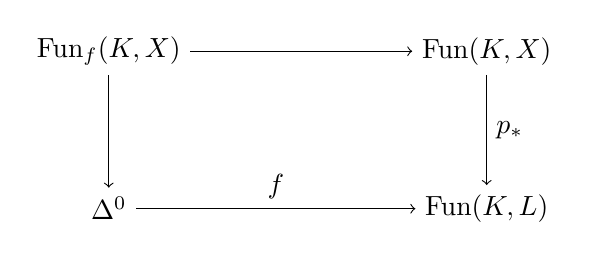
\begin{tikzpicture}
  \node (ff) at (0,0) {$\mathrm{Fun}_f(K, X)$};
  \node (f) at (4.8,0) {$\mathrm{Fun}(K, X)$};
  \node (d0) at (0,-2.0) {$\Delta^0$};
  \node (fl) at (4.8,-2.0) {$\mathrm{Fun}(K, L)$};
  \draw[->] (ff) -- (f);
  \draw[->] (f) -- node[right] {$p_*$} (fl);
  \draw[->] (d0) -- node[above] {$f$} (fl);
  \draw[->] (ff) -- (d0);
\end{tikzpicture}
\end{center}
若 $f = \mathrm{id}\colon L \to L$，则我们径直把 $\mathrm{Fun}_{\mathrm{id}}(K, X)$
写作 $\mathrm{Fun}_L(L, X)$。
\end{definition}

\begin{definition}\label{def:cofinal-coinitial}
设 $f\colon K \to L$ 是\trSimplicialSets{}的一个映射。若对一切\trRightFibration{}%
$p\colon X \to L$，\footnote{译注：原书此处印作「$p\colon X \to Y$」；按%
\cref{def:relative-fun-space}的记号，其靶应为 $L$，译文径改。
coinitial 情形的相应笔误同此处理。——译者注}由 $f$ 诱导的典范映射
\[
\mathrm{Fun}_L(L, X) \longrightarrow \mathrm{Fun}_f(K, X)
\]
是\trJoyalEquivalence{}，则称 $f$ 是\emph{\trCofinal{}}（cofinal）。同样地，
称 $f$ 是\emph{\trCoinitial{}}（coinitial），如果对一切\trLeftFibration{}%
$p\colon X \to L$，典范映射
\[
\mathrm{Fun}_L(L, X) \longrightarrow \mathrm{Fun}_f(K, X)
\]
是\trJoyalEquivalence{}。
\end{definition}

\begin{remark}\label{rem:fun-f-groupoid}
由构造，若 $p\colon X \to L$ 是一个\trRightFibration{}或\trLeftFibration{}，则
$\mathrm{Fun}_f(K, X)$ 是一个\trInfinityGroupoid{}；这是因为此时它到 $\Delta^0$
的典范映射是一个\trRightFibration{}或\trLeftFibration{}，从而是一个%
\trKanFibration{}。按我们先前的记号，「$p\colon \E \to \C$ 是∞-\trCategories{}之间
的一个\trLeftFibration{}」这一事实曾被写作
$\mathrm{Fun}^{\mathrm{cc}}_f(\C, \E^{\natural})$，因为对\trLeftFibration{}而言，
$\E$ 中的任何\trMorphism{}都是 $p$-余笛卡尔的。
\end{remark}

\begin{proposition}\label{prop:cofinal-composition}
设 $f\colon K \to L$ 与 $g\colon L \to M$ 是\trSimplicialSets{}的映射。
\begin{enumerate}[label=(\arabic*)]
  \item 若 $f$ 是\trCofinal{}，则 $gf$ 是\trCofinal{}当且仅当 $g$ 是。
  \item 若 $f$ 是\trCofinal{}，则 $f$ 是一个\trWeakEquivalence{}。
  \item 若 $f$ 是一个\trMonomorphism{}，则 $f$ 是\trCofinal{}当且仅当它是%
        \trRightAnodyne{}的。
\end{enumerate}
\end{proposition}

\begin{proof}
我们先证（1）。为此，考虑一个\trRightFibration{} $\D \to M$ 与图表
\begin{center}
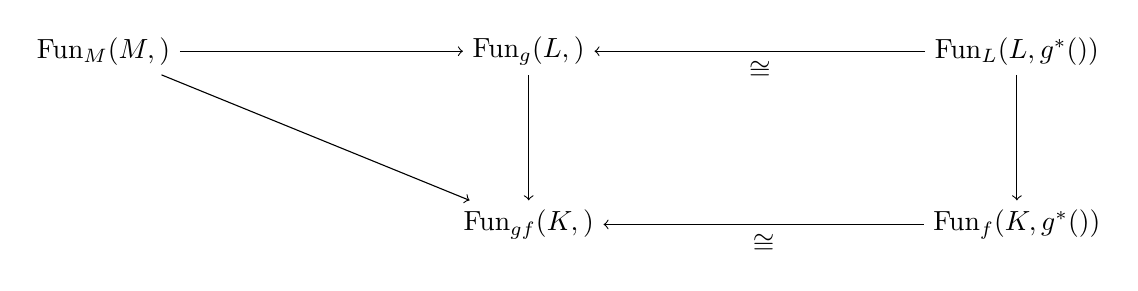
\begin{tikzpicture}
  \node (mm) at (0,0) {$\mathrm{Fun}_M(M, \D)$};
  \node (gg) at (5.4,0) {$\mathrm{Fun}_g(L, \D)$};
  \node (ll) at (11.6,0) {$\mathrm{Fun}_L(L, g^*(\D))$};
  \node (gf) at (5.4,-2.2) {$\mathrm{Fun}_{gf}(K, \D)$};
  \node (ff) at (11.6,-2.2) {$\mathrm{Fun}_f(K, g^*(\D))$};
  \draw[->] (mm) -- (gg);
  \draw[->] (ll) -- node[below] {$\cong$} (gg);
  \draw[->] (mm) -- (gf);
  \draw[->] (gg) -- (gf);
  \draw[->] (ll) -- (ff);
  \draw[->] (ff) -- node[below] {$\cong$} (gf);
\end{tikzpicture}
\end{center}
其中右侧的两个水平映射都是同构，而最右侧的竖直映射是\trJoyalEquivalence{}——
由 $f$ 是\trCofinal{}这一假设以及「\trRightFibration{}的\trPullback{}仍是%
\trRightFibration{}」这一事实即知。于是由\trThreeForTwoProperty{}即得本结论。

为了证明（2），只需证明：对任何\trKanComplex{} $X$，典范映射
$\mathrm{Fun}(L, X) \to \mathrm{Fun}(K, X)$ 是一个\trHomotopyEquivalence{}。考虑
映射 $L \times X \to L$，它是一个\trKanFibration{}，从而特别地是一个%
\trRightFibration{}。于是我们发现
$\mathrm{Fun}_L(L, L \times X) \cong \mathrm{Fun}(L, X)$，并且
$\mathrm{Fun}_f(K, L \times X) \cong \mathrm{Fun}(K, X)$，这正是所需要的。

为了看出\trRightAnodyne{}的映射是\trCofinal{}，我们断言：所要分析的那个限制
映射是一个\trTrivialFibration{}。具体地说，由\trAdjunction{}，只需证明：对任何%
\trMonomorphism{} $S \to T$，诱导映射
\[
S \times L \cup T \times K \longrightarrow T \times L
\]
也是\trRightAnodyne{}的，而这一点已在第 1 章中的\cref{lem:box-anodyne}中建立。反之，假设
$f$ 是\trCofinal{}\trMonomorphism{}，并设 $X \to Y$ 是一个\trRightFibration{}；
为判断 $f$ 是否\trRightAnodyne{}，考虑一个\trLiftingProblem{}。经\trPullback{}，
我们不妨设 $Y = L$，于是得到图表
\begin{center}
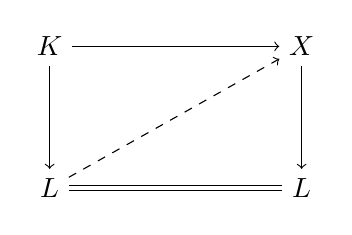
\begin{tikzpicture}
  \node (k) at (0,0) {$K$};
  \node (x) at (3.2,0) {$X$};
  \node (l1) at (0,-1.8) {$L$};
  \node (l2) at (3.2,-1.8) {$L$};
  \draw[->] (k) -- (x);
  \draw[->] (k) -- (l1);
  \draw[->] (x) -- (l2);
  \draw[double, double distance=1.2pt] (l1) -- (l2);
  \draw[->, dashed] (l1) -- (x);
\end{tikzpicture}
\end{center}
这时我们希望证明虚箭头的存在性。由假设，我们知道\trMorphism{}%
\[
\mathrm{Fun}_L(L, X) \to \mathrm{Fun}_f(K, X)
\]
是一个\trJoyalEquivalence{}。如果我们还能证明它同时是一个\trIsofibration{}，
那么由第 2 章中的\cref{lem:trivial-fibration-joyal-isofibration}，它是一个%
\trTrivialFibration{}，从而在 $0$-\trSimplex{}上是满的（这就证明了上述虚箭头的
存在性）。为了看出它确实是一个\trIsofibration{}，我们首先注意到它是一个%
\trInnerFibration{}——这里用到「\trInnerAnodyne{}映射与\trMonomorphism{}的%
\trPushoutProduct{}是\trInnerAnodyne{}的」以及「\trRightFibration{}特别地是%
\trInnerFibration{}」这两个事实。剩下的只需证明：任何图表
\begin{center}
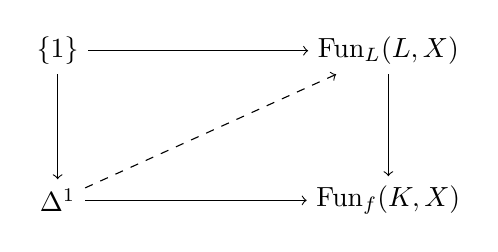
\begin{tikzpicture}
  \node (o) at (0,0) {$\{1\}$};
  \node (fl) at (4.2,0) {$\mathrm{Fun}_L(L, X)$};
  \node (d1) at (0,-1.9) {$\Delta^1$};
  \node (ff) at (4.2,-1.9) {$\mathrm{Fun}_f(K, X)$};
  \draw[->] (o) -- (fl);
  \draw[->] (o) -- (d1);
  \draw[->] (d1) -- (ff);
  \draw[->] (fl) -- (ff);
  \draw[->, dashed] (d1) -- (fl);
\end{tikzpicture}
\end{center}
都容有一条使图表交换的虚箭头。而这是对的，因为右侧的竖直映射是%
\trConservative{}（作为∞-\trGroupoid{}之间的一个\trFunctor{}）。现在我们
利用「\trRightAnodyne{}映射与\trMonomorphism{}的\trPushoutProduct{}仍是%
\trRightAnodyne{}的」这一事实；于是，由 $X \to L$ 是\trRightFibration{}，提升
存在。
\end{proof}

\begin{corollary}\label{cor:coinitial-dual}
设 $f\colon K \to L$ 与 $g\colon L \to M$ 是\trSimplicialSets{}的映射。
\begin{enumerate}[label=(\arabic*)]
  \item 若 $f$ 是\trCoinitial{}，则 $gf$ 是\trCoinitial{}当且仅当 $g$ 是%
        \trCoinitial{}。
  \item 若 $f$ 是一个\trMonomorphism{}，则 $f$ 是\trCoinitial{}当且仅当 $f$
        是\trLeftAnodyne{}的。
\end{enumerate}
\end{corollary}

\begin{proof}
这由\cref{ex:cofinal-coinitial-op}立即得出。
\end{proof}

\begin{corollary}\label{cor:right-cancellation}
在诸\trMonomorphism{}之中，\trLeftAnodyne{}映射与\trRightAnodyne{}映射满足
右消去性质（right-cancellation property）：若 $f$ 与 $g$ 是可合成的%
\trMorphism{}，并且
$f$ 与 $gf$ 二者同为\trLeftAnodyne{}的或同为\trRightAnodyne{}的，则同样的结论
对 $g$ 成立。
\end{corollary}

接下来，我们想证明\trCofinal{}映射的一个重要刻画，它建立在下述引理之上。

\begin{lemma}\label{lem:tilde-map-slice-cartesian}
设 $F\colon L \to \C$ 是一个图表，$x$ 是 $\C$ 的一个\trObject{}。那么，存在如下
一个典范的笛卡尔（并且\trHomotopyCartesian{}）图表：
\begin{center}
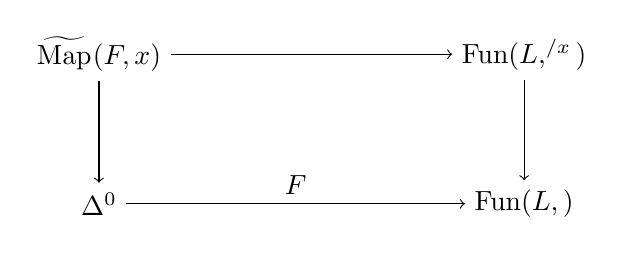
\begin{tikzpicture}
  \node (m) at (0,0) {$\widetilde{\mathrm{Map}}_{\C}(F, x)$};
  \node (fs) at (5.4,0) {$\mathrm{Fun}(L, \C^{/x})$};
  \node (d0) at (0,-1.9) {$\Delta^0$};
  \node (fl) at (5.4,-1.9) {$\mathrm{Fun}(L, \C)$};
  \draw[->] (m) -- (fs);
  \draw[->] (m) -- (d0);
  \draw[->] (fs) -- (fl);
  \draw[->] (d0) -- node[above] {$F$} (fl);
\end{tikzpicture}
\end{center}
\end{lemma}

\begin{proof}
同样地，在证明期间我们姑且把这个\trPullback{}称为 $\Phi(F)$。注意到，从一个%
\trSimplicialSet{} $X$ 到 $\Phi(F)$ 的一个映射对应于一个映射
\[
[(X \times L) \diamond \Delta^0] \amalg_{X \times L} L \longrightarrow \C,
\]
它到 $\Delta^0$ 的限制由 $x$ 给出，而它到 $L$ 的限制是 $F$。另一方面，从 $X$ 到
$\widetilde{\mathrm{Map}}_{\C}(F, x)$ 的一个映射对应于一个映射
\[
[X \times (L \diamond \Delta^0)]
  \amalg_{X \times (L \cup \{\infty\})} L \cup \{\infty\}
  \longrightarrow \C,
\]
它到 $L \cup \{\infty\}$ 的限制是偶对 $(F, x)$。我们断言，存在\trSimplicialSets{}%
之间的一个同构
\[
[(X \times L) \diamond \Delta^0] \amalg_{X \times L} L
  \cong [X \times (L \diamond \Delta^0)]
        \amalg_{X \times (L \cup \{\infty\})} L \cup \{\infty\}.
\]
为此，我们如下计算：
\[
\begin{aligned}
[(X \times L) \diamond \Delta^0] \amalg_{X \times L} L
&\cong \bigl[(X \times L \times \Delta^1)
  \amalg_{X \times L \times \partial\Delta^1} (X \times L) \amalg \Delta^0\bigr]
  \amalg_{X \times L} L \\
&\cong (X \times L \times \Delta^1)
  \amalg_{X \times L \times \partial\Delta^1} \\
&\qquad \bigl((X \times L) \amalg \Delta^0
  \amalg_{X \times L} L\bigr) \\
&\cong (X \times L \times \Delta^1)
  \amalg_{X \times L \times \partial\Delta^1} L \amalg \Delta^0 \\
&\cong (X \times L \times \Delta^1)
  \amalg_{X \times L \times \partial\Delta^1} \\
&\qquad \bigl(X \times (L \amalg \Delta^0)
  \amalg_{X \times (L \amalg \Delta^0)} L \amalg \Delta^0\bigr) \\
&\cong \bigl((X \times L \times \Delta^1)
  \amalg_{X \times L \times \partial\Delta^1} X \times (L \amalg \Delta^0)\bigr) \\
&\qquad \amalg_{X \times (L \amalg \Delta^0)} L \amalg \Delta^0 \\
&\cong X \times (L \diamond \Delta^0)
  \amalg_{X \times (L \amalg \Delta^0)} L \amalg \Delta^0
\end{aligned}
\]
这样便证得本引理，只要我们让自己确信 $\Delta^0$ 与 $L$ 的诸包含映射相互对应
（这无非是核对若干映射的简单事务）。
\end{proof}

\begin{theorem}\label{thm:cofinal-characterization}
设 $f\colon K \to L$ 是\trSimplicialSets{}的一个映射。那么，$f$ 是\trCofinal{}，
当且仅当对每个∞-\trCategory{} $\C$ 与每个图表 $p\colon L \to \C$，诱导映射
$\C^{p/} \to \C^{pf/}$ 是一个\trJoyalEquivalence{}。
\end{theorem}

\begin{proof}
我们先假设 $f$ 是\trCofinal{}，并证明此时映射 $\C^{p/} \to \C^{pf/}$ 是一个%
\trJoyalEquivalence{}。由于该映射是 $\C$ 上的若干\trLeftFibration{}之间的一个
映射，只需证明：它在\trObject{} $x \in \C$ 上的纤维处诱导的映射是一个%
\trEquivalence{}。由\cref{lem:tilde-map-slice-cartesian}，这个映射（在%
\trHomotopyEquivalence{}的意义下）可以等同于映射
$\mathrm{Fun}_p(L, \C^{/x}) \to \mathrm{Fun}_{pf}(K, \C^{/x})$，而后者是一个%
\trEquivalence{}，因为 $\C^{/x} \to \C$ 是一个\trRightFibration{}且 $f$ 是%
\trCofinal{}。反之，假设对任何图表 $p\colon L \to \C$，映射
$\C^{p/} \to \C^{pf/}$ 都是一个\trJoyalEquivalence{}，并设 $X \to L$ 是一个%
\trRightFibration{}。由\trStraightening{}--\trUnstraightening{}\trEquivalence{}，
存在一个\trFunctor{} $p\colon L \to \mathrm{Spc}^{\mathrm{op}}$，使得泛%
\trRightFibration{}沿它的\trPullback{}等价于 $X \to L$。现在我们利用「泛%
\trRightFibration{}由
$(\mathrm{Spc}_*/)^{\mathrm{op}} \to \mathrm{Spc}^{\mathrm{op}}$ 给出」这一事实；
由于
$(\mathrm{Spc}_*/)^{\mathrm{op}} \simeq (\mathrm{Spc}^{\mathrm{op}})_{/*}$，它是一
个\trRepresentable{}\trRightFibration{}。于是，利用%
\cref{lem:tilde-map-slice-cartesian}，我们发现
\[
\mathrm{Fun}_L(L, X) \simeq \mathrm{Fun}_p(L, (\mathrm{Spc}_*/)^{\mathrm{op}})
  \simeq \mathrm{Map}_{\mathrm{Spc}^{\mathrm{op}}}(p, *)
  \simeq (\mathrm{Spc}^{\mathrm{op}})^{p/}
  \times_{\mathrm{Spc}^{\mathrm{op}}} \{*\},
\]
并且同样地
\[
\mathrm{Fun}_f(K, X) \simeq (\mathrm{Spc}^{\mathrm{op}})^{pf/}
  \times_{\mathrm{Spc}^{\mathrm{op}}} \{*\}.
\]
我们所要考察的映射，是由 $\mathrm{Spc}^{\mathrm{op}}$ 上的诸\trLeftFibration{}%
$(\mathrm{Spc}^{\mathrm{op}})^{p/} \to (\mathrm{Spc}^{\mathrm{op}})^{pf/}$
取 $* \in \mathrm{Spc}^{\mathrm{op}}$ 上的%
\trFibre{}而诱导的那个映射。由假设，该映射是一个\trJoyalEquivalence{}，从而在
纤维上诱导的映射也是一个\trJoyalEquivalence{}。
\end{proof}

\begin{corollary}\label{cor:joyal-equiv-cofinal}
任何\trJoyalEquivalence{} $f\colon K \to L$ 都是\trCofinal{}。
\end{corollary}

\begin{proof}
由\cref{thm:cofinal-characterization}，只需证明：对每个∞-\trCategory{} $\C$ 与
每个图表，诱导映射 $\C^{p/} \to \C^{pf/}$ 是一个\trJoyalEquivalence{}。为此，
只需证明：对再一个∞-\trCategory{} $\D$，诱导映射
\[
\mathrm{Fun}(\D, \C^{p/}) \longrightarrow \mathrm{Fun}(\D, \C^{pf/})
\]
是一个\trEquivalence{}。由\trAdjunction{}，该映射同构于
\[
\mathrm{Fun}_p(\D \diamond L, \C) \longrightarrow
  \mathrm{Fun}_{pf}(\D \diamond K, \C),
\]
而后者又由下述图表中\trPullback{}上的诱导映射给出：
\begin{center}
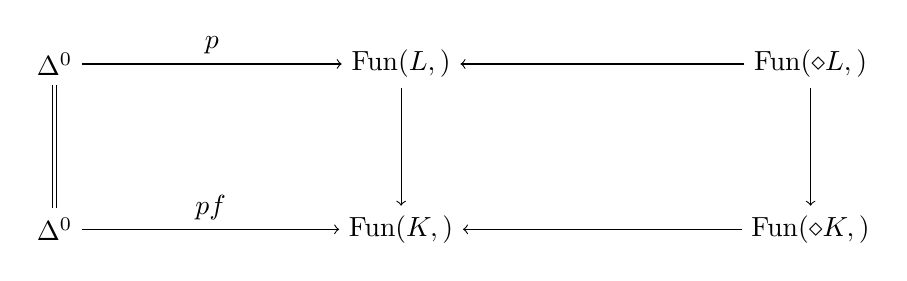
\begin{tikzpicture}
  \node (d0a) at (0,0) {$\Delta^0$};
  \node (fl) at (4.4,0) {$\mathrm{Fun}(L, \C)$};
  \node (fdl) at (9.6,0) {$\mathrm{Fun}(\D \diamond L, \C)$};
  \node (d0b) at (0,-2.1) {$\Delta^0$};
  \node (fk) at (4.4,-2.1) {$\mathrm{Fun}(K, \C)$};
  \node (fdk) at (9.6,-2.1) {$\mathrm{Fun}(\D \diamond K, \C)$};
  \draw[->] (d0a) -- node[above] {$p$} (fl);
  \draw[->] (fdl) -- (fl);
  \draw[->] (d0b) -- node[above] {$pf$} (fk);
  \draw[->] (fdk) -- (fk);
  \draw[double, double distance=1.2pt] (d0a) -- (d0b);
  \draw[->] (fl) -- (fk);
  \draw[->] (fdl) -- (fdk);
\end{tikzpicture}
\end{center}
其中右侧的两个水平映射是\trIsofibration{}，而全部竖直映射都是%
\trJoyalEquivalence{}（就右侧而言，这由第 2 章中的\cref{cor:fat-join-joyal-equivalence}
得到：$\D \diamond K \to \D \diamond L$ 仍是一个\trJoyalEquivalence{}）。于是，
由第 2 章中的\cref{lem:pullback-joyal-equivalence}，\trPullback{}上的诱导映射也是一个%
\trJoyalEquivalence{}。
\end{proof}

\begin{corollary}\label{cor:cofinal-colimit}
设 $f\colon K \to L$ 是一个\trCofinal{}映射，并设 $p\colon L \to \C$ 是一个%
图表，其中 $\C$ 是一个∞-\trCategory{}。那么，$p$ 容许一个\trColimit{}当且仅当
$pf$ 容许一个\trColimit{}，并且在任一情形下，$p$ 保持这个\trColimit{}。
\footnote{译注：原书此两处均印作「$f$ 容许／保持」；按上下文应为图表 $p$
（$f\colon K \to L$ 不是 $\C$ 值图表，谈不上容有或保持\trColimit{}），译文径改。
——译者注}
\end{corollary}

\begin{lemma}\label{lem:trivial-fibration-cofinal-right}
设 $f\colon K \to L$ 是\trSimplicialSets{}的一个映射。那么，$f$ 是一个%
\trTrivialFibration{}当且仅当它是一个\trCofinal{}\trRightFibration{}。
\end{lemma}

\begin{proof}
「仅当」部分由「\trTrivialFibration{}既是\trRightFibration{}又是%
\trJoyalEquivalence{}」这一事实得出。为了看出反方向，我们将证明诸\trFibre{}是%
\trContractible{}，然后援引\cref{ex:cocartesian-trivial-fibration}的对偶版本。设 $K \to L$ 是一个%
\trCofinal{}\trRightFibration{}。那么，映射
\[
\mathrm{Fun}_L(L, K) \to \mathrm{Fun}_f(K, K)
\]
是一个\trEquivalence{}。右边含有\trFunctor{}%
$\mathrm{id}_K\colon K \to K$，故存在一个\trObject{}%
$\varphi\colon \Delta^0 \to \mathrm{Fun}_L(L, K)$，它在
$\mathrm{Fun}_f(K, K)$ 中的像等价于 $\mathrm{id}_K$。\footnote{译注：原书此处
印作「$\Delta^0 \to \mathrm{Fun}_L(L, X)$」；按上下文，其靶应为
$\mathrm{Fun}_L(L, K)$，译文径改。——译者注}把它明写出来，我们便得到
$f\varphi = \mathrm{id}_L$，并且存在一条连接 $\mathrm{id}_K$ 与 $\varphi f$
的 $1$-\trSimplex{} $\Delta^1 \to \mathrm{Fun}_f(K, K)$。这对应于一个交换图表
\begin{center}
\begin{tikzpicture}
  \node (dk) at (0,0) {$\Delta^1 \times K$};
  \node (k1) at (3.8,0) {$K$};
  \node (k2) at (0,-1.9) {$K$};
  \node (l) at (3.8,-1.9) {$L$};
  \draw[->] (dk) -- node[above] {$h$} (k1);
  \draw[->] (dk) -- node[left] {$\mathrm{pr}$} (k2);
  \draw[->] (k1) -- node[right] {$f$} (l);
  \draw[->] (k2) -- node[above] {$f$} (l);
\end{tikzpicture}
\end{center}
于是，对 $L$ 的任何 $0$-\trSimplex{} $x$，我们可以把映射 $h$ 限制到
$\Delta^1 \times K_x$ 上。容易看出，所得的映射给出了 $\mathrm{id}_K$ 与
$\varphi f$ 限制在 $K_x$ 上的一个\trHomotopy{}。后者是常值映射，因为 $f$ 在诸
纤维上是常值的。这样，每个\trFibre{} $K_x$ 都是一个\trContractible{}%
\trKanComplex{}。
\end{proof}

\begin{proposition}\label{prop:cofinal-factorization}
一个映射是\trCofinal{}，当且仅当它是一个\trRightAnodyne{}映射后接一个%
\trTrivialFibration{}的复合。
\end{proposition}

\begin{proof}
「若」的情形是清楚的：\trRightAnodyne{}映射与\trTrivialFibration{}都是%
\trCofinal{}，而且\trCofinal{}映射的复合仍是\trCofinal{}。反之，给定一个%
\trCofinal{}映射 $f\colon K \to L$，我们可以把它分解为一个\trRightAnodyne{}%
映射 $K \to K'$ 后接一个\trRightFibration{} $K' \to L$。由于\trRightAnodyne{}%
映射是\trCofinal{}，由\cref{prop:cofinal-composition}的（1），\trRightFibration{}%
$K' \to L$ 是\trCofinal{}。于是，断言由\cref{lem:trivial-fibration-cofinal-right}
得出。
\end{proof}

\begin{definition}\label{def:smooth-proper}
设 $p\colon Y \to X$ 是\trSimplicialSets{}的一个映射。如果对每个\trPullback{}图表
\begin{center}
\begin{tikzpicture}
  \node (b) at (0,0) {$B$};
  \node (y) at (2.8,0) {$Y$};
  \node (a) at (0,-1.8) {$A$};
  \node (x) at (2.8,-1.8) {$X$};
  \draw[->] (b) -- node[above] {$j$} (y);
  \draw[->] (b) -- (a);
  \draw[->] (y) -- node[right] {$p$} (x);
  \draw[->] (a) -- node[above] {$i$} (x);
\end{tikzpicture}
\end{center}
（其中 $i$ 是\trCofinal{}），映射 $j$ 都仍是\trCofinal{}，我们就称 $p$ 是%
\emph{\trSmooth{}}。对偶地，如果对每个这类\trPullback{}图表（其中 $i$
是\trCoinitial{}），映射 $j$ 都仍是\trCoinitial{}，我们就称它是%
\emph{\trProper{}}。
\end{definition}

\begin{definition}\label{def:universally-smooth-proper}
\trSimplicialSets{}的一个映射 $p\colon Y \to X$ 称为%
\emph{\trUniversallySmooth{}}（universally smooth），如果沿任何映射
$X' \to X$ 取\trPullback{}都得到\trSmooth{}映射。同样地，
称它是\emph{\trUniversallyProper{}}（universally proper），如果沿任何映射取%
\trPullback{}都得到\trProper{}映射。
\end{definition}

\begin{remark}\label{rem:terminology-warning}
关于文献中的不同术语，有必要提醒几句。在 \cite{Lur09} 中，我们所称的%
\trUniversallySmooth{}被径直称作\trSmooth{}，\trProper{}与%
\trUniversallyProper{}这两个词亦然。我们之所以要作这一区分，是因为%
\trUniversallyProper{}映射沿\trPullback{}封闭，而（按我们的术语）\trProper{}%
映射并不沿\trPullback{}封闭，见\cref{ex:proper-not-universally-proper}。在 \cite{Cis19,Ngu18} 中，我们所称的%
\trUniversallySmooth{}被称作\trProper{}，而我们所称的\trUniversallyProper{}被
称作\trSmooth{}。事实上，这套分歧还要出现得更早一些：我们所称的\trCofinal{}在
那里被称作终的（final），我们所称的\trCoinitial{}在那里被称作共尾的（cofinal），而我们所称的%
\trSmooth{}或\trProper{}在 \cite{Cis19,Ngu18} 中并没有单独的名称。
\end{remark}

对于下面的命题，我们沿用 \cite[2.3.23]{Ngu18} 与 \cite{Cis19} 中给出的证明。

\begin{proposition}\label{prop:base-change-right-anodyne}
考虑\trPullback{}图表
\begin{center}
\begin{tikzpicture}
  \node (b) at (0,0) {$B$};
  \node (y) at (2.8,0) {$Y$};
  \node (a) at (0,-1.8) {$A$};
  \node (x) at (2.8,-1.8) {$X$};
  \draw[->] (b) -- node[above] {$j$} (y);
  \draw[->] (b) -- (a);
  \draw[->] (y) -- node[right] {$p$} (x);
  \draw[->] (a) -- node[above] {$i$} (x);
\end{tikzpicture}
\end{center}
其中 $p$ 是一个\trLeftFibration{}而 $i$ 是\trRightAnodyne{}的。那么，映射 $j$
仍是\trRightAnodyne{}的。
\end{proposition}

\begin{proof}
第一步是注意到：只需对 $i$ 含于\trRightAnodyne{}映射的某个生成集之中的情形证明本
断言。为此，我们断言：由满足本命题结论的那些\trRightAnodyne{}映射组成的集合 $S$
是\trSaturated{}，见\cref{ex:right-anodyne-pullback-saturated}。虽然对复合与收缩而言这一点容易看出，但要看出这些
映射沿推出封闭，还需稍费些工夫。由第 1 章中的\cref{cor:right-box-generators}，届时只需证明
映射
$\{1\} \times \Delta^n \cup \Delta^1 \times \partial\Delta^n \to \Delta^1 \times \Delta^n$
含于此集合之中。同样注意到，集合 $S$ 具有右消去性质，因为按\cref{ex:right-anodyne-pullback-saturated}，一切%
\trRightAnodyne{}映射都有这一性质。于是，只需证明：对任何\trSimplicialSet{} $K$，
映射
\[
\{1\} \times K \to \Delta^1 \times K
\]
含于 $S$ 中。为此，考虑图表
\begin{center}
\begin{tikzpicture}
  \node (tl) at (0,0) {$\{1\} \times \partial\Delta^n$};
  \node (tr) at (5.6,0) {$\Delta^1 \times \partial\Delta^n$};
  \node (ml) at (0,-2.1) {$\{1\} \times \Delta^n$};
  \node (mr) at (5.6,-2.1)
    {$\{1\} \times \Delta^n \cup \Delta^1 \times \partial\Delta^n$};
  \node (br) at (11.0,-3.9) {$\Delta^1 \times \Delta^n$};
  \draw[->] (tl) -- (tr);
  \draw[->] (tl) -- (ml);
  \draw[->] (ml) -- (mr);
  \draw[->] (tr) -- (mr);
  \draw[->] (tr) to[bend left=20] (br);
  \draw[->] (ml) to[bend right=12] (br);
  \draw[->] (mr) -- (br);
\end{tikzpicture}
\end{center}
利用上述断言，我们发现上方的水平映射含于 $S$ 中。于是，由于 $S$ 沿推出封闭，
下方的水平映射亦然。此外，下方的弯曲映射含于 $S$ 中。由于 $S$ 满足右消去性质，
对角映射也含于 $S$ 中。

现在我们观察到，映射 $\{1\} \times K \to \Delta^1 \times K$ 是\trRightAnodyne{}%
扩张（right-anodyne extension）的特例：也就是说，它们是右形变收缩（right
deformation retract），而\cref{ex:right-deformation-retract}证明了右形变收缩沿\trLeftFibration{}的%
\trPullback{}是封闭的。
\end{proof}

\begin{remark}\label{rem:base-change-left-anodyne}
通过应用\trOppositeFunctor{}，我们发现：若 $p$ 是一个\trRightFibration{}而 $i$
是\trLeftAnodyne{}的，则 $j$ 仍是\trLeftAnodyne{}的。
\end{remark}

\begin{remark}\label{rem:base-change-cocartesian}
\cref{prop:base-change-right-anodyne}的结论对\trCocartesianFibration{}%
$p\colon Y \to X$ 而言更一般地成立，见 \cite[Proposition 4.1.2.15]{Lur09}。
\end{remark}

\begin{corollary}\label{cor:left-fibration-smooth}
\trLeftFibration{}都是\trUniversallySmooth{}。事实上，\trCocartesianFibration{}%
都是\trUniversallySmooth{}。\trRightFibration{}——事实上，
\trCartesianFibration{}——都是\trUniversallyProper{}。
\end{corollary}

\begin{proof}
由于\trLeftFibration{}与\trRightFibration{}沿\trPullback{}封闭，只需证明一个%
\trLeftFibration{}是\trSmooth{}。为此，考虑一个如\trSmooth{}映射之定义中的图表，
把映射 $i$
分解为
\[
A \xrightarrow{\ i'\ } A' \xrightarrow{\ p\ } X,
\]
其中 $i'$ 是\trRightAnodyne{}的而 $p$ 是一个\trTrivialFibration{}，并考虑扩大后
的图表
\begin{center}
\begin{tikzpicture}
  \node (b) at (0,0) {$B$};
  \node (bp) at (3.4,0) {$B'$};
  \node (y) at (6.8,0) {$Y$};
  \node (a) at (0,-1.9) {$A$};
  \node (ap) at (3.4,-1.9) {$A'$};
  \node (x) at (6.8,-1.9) {$X$};
  \draw[->] (b) -- node[above] {$j'$} (bp);
  \draw[->] (bp) -- node[above] {$q$} (y);
  \draw[->] (b) -- (a);
  \draw[->] (bp) -- (ap);
  \draw[->] (y) -- (x);
  \draw[->] (a) -- (ap);
  \draw[->] (ap) -- (x);
\end{tikzpicture}
\end{center}
我们发现 $q$ 是一个\trTrivialFibration{}，而由\cref{prop:base-change-right-anodyne}，
$j'$ 是\trRightAnodyne{}的。于是，$j$ 作为\trCofinal{}映射的复合是\trCofinal{}。
\end{proof}

利用「\trLeftFibration{}是\trSmooth{}而\trRightFibration{}是\trProper{}」这一
事实，我们便
得到 \trQuillen{}定理 A 的\trInfinityCategory{}版本的一个漂亮证明。注意，该定理
为那些靶是∞-\trCategory{}的映射提供了关于\trCofinality{}（cofinality）的又一个
刻画。

\begin{theorem}\label{thm:quillen-theorem-a}
设 $f\colon \C \to \D$ 是\trSimplicialSets{}的一个映射，其中 $\D$ 是一个∞-%
\trCategory{}。那么，$f$ 是\trCofinal{}，当且仅当对 $\D$ 的一切\trObject{} $d$，
\trSimplicialSet{} $\C_{d/}$ 是\trWeaklyContractible{}。
\end{theorem}

\begin{proof}
首先，假设 $f$ 是\trCofinal{}。在\trPullback{}图表
\begin{center}
\begin{tikzpicture}
  \node (cd) at (0,0) {$\C_{d/}$};
  \node (dd) at (3.6,0) {$\D_{d/}$};
  \node (c) at (0,-1.9) {$\C$};
  \node (d) at (3.6,-1.9) {$\D$};
  \draw[->] (cd) -- (dd);
  \draw[->] (cd) -- (c);
  \draw[->] (dd) -- (d);
  \draw[->] (c) -- (d);
\end{tikzpicture}
\end{center}
中，右侧的竖直映射是一个\trLeftFibration{}，从而是\trSmooth{}。由此可知，
$\C_{d/} \to \D_{d/}$ 是\trCofinal{}，从而是一个\trWeakEquivalence{}。由于
$\D_{d/}$ 是\trWeaklyContractible{}（它有一个\trInitialObject{}），同样的结论
对 $\C_{d/}$ 成立。

对于反方向，我们考虑 $f$ 的一个分解
\[
\C \xrightarrow{\ i\ } \E \xrightarrow{\ p\ } \D
\]
其中 $i$ 是\trRightAnodyne{}的而 $p$ 是一个\trRightFibration{}。我们想证明 $p$
是一个\trTrivialFibration{}，从而由\cref{prop:cofinal-factorization}知 $f$ 是%
\trCofinal{}。为此，考虑图表
\begin{center}
\begin{tikzpicture}
  \node (cd) at (0,0) {$\C_{d/}$};
  \node (ed) at (3.8,0) {$\E_{d/}$};
  \node (dd) at (7.6,0) {$\D_{d/}$};
  \node (c) at (0,-1.9) {$\C$};
  \node (e) at (3.8,-1.9) {$\E$};
  \node (d) at (7.6,-1.9) {$\D$};
  \draw[->] (cd) -- (ed);
  \draw[->] (ed) -- (dd);
  \draw[->] (cd) -- (c);
  \draw[->] (ed) -- (e);
  \draw[->] (dd) -- (d);
  \draw[->] (c) -- (e);
  \draw[->] (e) -- (d);
\end{tikzpicture}
\end{center}
其中所有方块都是\trPullback{}。由于最右边的竖直映射是一个\trLeftFibration{}，
中间的竖直映射也是一个\trLeftFibration{}。由\cref{prop:base-change-right-anodyne}，
映射 $\C_{d/} \to \E_{d/}$ 仍是\trRightAnodyne{}的，从而是一个%
\trWeakEquivalence{}，于是 $\E_{d/}$ 是\trWeaklyContractible{}。

现在考虑图表
\begin{center}
\begin{tikzpicture}
  \node (ed) at (0,0) {$\E_d$};
  \node (eds) at (3.8,0) {$\E_{d/}$};
  \node (e) at (7.6,0) {$\E$};
  \node (d0) at (0,-1.9) {$\Delta^0$};
  \node (dd) at (3.8,-1.9) {$\D_{d/}$};
  \node (d) at (7.6,-1.9) {$\D$};
  \draw[->] (ed) -- (eds);
  \draw[->] (eds) -- (e);
  \draw[->] (ed) -- (d0);
  \draw[->] (eds) -- (dd);
  \draw[->] (e) -- (d);
  \draw[->] (d0) -- node[above] {$\mathrm{id}_d$} (dd);
  \draw[->] (dd) -- (d);
\end{tikzpicture}
\end{center}
同样，所有方块都是\trPullback{}。这一次，最右边的竖直映射是一个%
\trRightFibration{}，故中间的竖直映射也是\trRightFibration{}。此外，映射
$\Delta^0 \to \D_{d/}$ 由\cref{lem:initial-left-anodyne}是\trLeftAnodyne{}的，
因为 $\mathrm{id}_d$ 是
$\D_{d/}$ 的一个\trInitialObject{}（见\cref{ex:terminal-object-slice}）。于是，由%
\cref{prop:base-change-right-anodyne}的对偶版本，映射 $\E_d \to \E_{d/}$ 是%
\trLeftAnodyne{}的，从而是一个\trWeakEquivalence{}。由于 $\E_{d/}$ 由第一步已知
是\trWeaklyContractible{}，而 $\E_d$ 是一个\trInfinityGroupoid{}，这就意味着%
\trRightFibration{} $p\colon \E \to \D$ 的诸\trFibre{} $\E_d$ 都是%
\trContractible{}。于是，$p$ 是一个\trTrivialFibration{}，例如由\cref{ex:cocartesian-trivial-fibration}便可
得知。
\end{proof}

\begin{remark}\label{rem:coinitial-criterion}
对偶地，\trSimplicialSets{}的一个映射 $F\colon \C \to \D$——其中 $\D$ 是一个
∞-\trCategory{}——是\trCoinitial{}，当且仅当对 $\D$ 的一切\trObject{} $d$，
\trSimplicialSet{} $\C_{/d}$ 是\trWeaklyContractible{}。
\end{remark}

为本章作结，下面便是 \trQuillen{}当年实际证明的那条陈述。
\footnote{译注：按 \trQuillen{}原文，定理 A 的假设是对每个 $d$，\trSliceCategory{}%
$F/d$——其\trObject{}为偶对 $(c, Fc \to d)$，即本书记号下的 $\C_{/d}$——的分类
空间是\trContractible{}；也就是说，原版对应的是\cref{rem:coinitial-criterion}
的 coinitial 准则。本推论把假设换成了其对偶——「$\C_{d/}$
\trWeaklyContractible{}」——由本节所证同样能推出 $\mathrm{N}(F)$ 是一个%
\trWeakEquivalence{}。——译者注}

\begin{corollary}\label{cor:quillen-theorem-a-original}
设 $F\colon \C \to \D$ 是\trOrdinaryCategory{}之间的一个\trFunctor{}。若全部
切片 $\C_{d/}$ 都是\trWeaklyContractible{}，则\trFunctor{}%
$\mathrm{N}(\C) \to \mathrm{N}(\D)$ 是一个\trWeakEquivalence{}。
\end{corollary}

\begin{proof}
由\cref{thm:quillen-theorem-a}，\trFunctor{}%
$\mathrm{N}(F)\colon \mathrm{N}(\C) \to \mathrm{N}(\D)$ 是\trCofinal{}，从而由%
\cref{prop:cofinal-composition}它是一个\trWeakEquivalence{}。
\end{proof}
